% Бүлэг 2

\pagecolor{ChapterYellow}
\chapter{Шаардлага ба шинжилгээ} % 2р бүлгийн гарчиг

\label{Chapter2} % Энэ бүлэг рүү ишлэл хийх бол \ref{Chapter2} командыг ашигла
%-------------------------------------------------------------------------------
%	SECTION 1
%-------------------------------------------------------------------------------
\pagecolor{white}
\section{Системийн үйл ажиллагаа}

Систем нь ямар нэг үйлчилгээний компанид зориулагдаагүй бөгөөд хүргэлтийн үйлчилгээ үзүүлдэг болон хувь хүн бүрд зориулагдсан ухаалаг систем юм. Системийг ашиглахын тулд хэрэглэгч интернет сүлжээнд холбогдсон байх ба системд бүртгэлтэй байх ёстой бөгөөд бүртгэлээ сошиал хаягаараа нээх аль эсвэл бүртгүүлэх форумыг бөглөж бүртгүүлнэ. Систем нь хүргэгч болон үйлчлүүлэгч гэсэн үндсэн хоёр хэрэглэгчтэй. Үйлчлүүлэгч нь хүргүүлэх үйлчилгээг өөрийн байгаа байршил дээр захиалж болно.\\
\textit{\textbf{Хүргэлтийн үйлчилгээ захиалах:}}\\
Хэрэглэгч хүргэлтийн мэдээллүүдээ системд оруулна ингэснээр захиалгыг бүртгэх ба хүргэгч нийт захиалга дундаас өөрийн хүссэн захиалгыг сонгон хүргэх боломжтой.\\
\textit{\textbf{Хүргэлтийн үйлчилгээ цуцлах:}}\\
Хэрэв хүргэлтийг хүргэж эхлээгүй бол хэрэглэгч үйлчилгээгээ цуцлаж хүргүүлэх хүсэлтээ устгах боломжтой.\\
\textit{\textbf{Хүргэлтийн үйлчилгээг дуусгах:}}\\
Хүргэгч хэрэв хүргэлтийг хүргэж өгсөн бол хүргэлтийг дуусгасан гэж тэмдэглэнэ.\\
\textit{\textbf{Хүргэгчийг үнэлэж оноо өгөх:}}\\
Хүргэгч хүргэлтийг хүргэж өгсөн бол үйлчлүүлэгч хүргэгчид үнэлгээ өгөх эрхтэй болно.\\
\textit{\textbf{Хэрэглэгчийн мэдээлэл шинэчлэх:}}\\
Хэрэглэгч систем өөрийн утас болон зураг нэрийг оруулах бөгөөд эдгээр мэдээллүүдийг дараа нь шинэчлэх боломжтой байна.

%-----------------------------------
%	SECTION 2
%-----------------------------------

\section{Системийг ашиглах хэрэглэгчид}

\subsection{Системийн оролцогч}
\begin{enumerate} 
    \item \textit{Хэрэглэгчид} - Системээр дамжуулан хүргэлтийн үйлчилгээг авах, эсвэл хүргэлтийн үйлчилгээ үзүүлэх хүсэлтэй хувь хүмүүс.
\end{enumerate}

\subsection{Системийн тоглогч}
\begin{enumerate}
    \item \textit{Үйлчлүүлэгч} - Системээр дамжуулан хүргэлтийн үйлчилгээг авах хүсэлтэй иргэн.
    \item \textit{Хүргэгч} - Системээр дамжуулан хүргэлтийн үйлчилгээ үзүүлэх хүсэлтэй иргэн.
\end{enumerate}

%-----------------------------------
%	SECTION 3
%-----------------------------------

\section{Функцийн шаардлага}

\begin{enumerate}
    \item Систем нь үйлчлүүлэгч болон жолооч гэсэн үндсэн 2 модультай байна.
    \item Хэрэглэгч хувийн мэдээллээ оруулан системд бүртгүүлнэ.
    \item Хэрэглэгч нь сошиал хаягаараа нэвтрэх орох боломжтой байна.
    \item Систем нь үйлчилгээ дууссаны дараа жолооч болон үйлчлүүлэгчдийн харилцаа үйлчилгээний үнэлгээг 1-ээс 5 одоор болон текст хэлбэрээр үнэлгээг авдаг байна.
    \item Системд хэрэглэгчээр бүртгүүлэхдээ нэр, зураг болон утасны дугаараа бүртгүүлнэ.
    \item Систем нь хүргэгчид хүргэлтийн цэг рүү очих хамгийн богино замыг зааж харуулдаг байна.
    \item Хүргэгч нь үйлчлүүлэгчийн захиалгыг гүйцэтгэсний дараа үйлчлүүлэгч үнэлгээ өгдөг байна.
\end{enumerate}
%-----------------------------------
%	SECTION 4
%-----------------------------------

\section{Функцийн бус шаардлага}
\begin{itemize}
	\item Гүйцэтгэлийн шаардлага:
	\begin{enumerate}
		\item Хурдан ажилладаг байх;
		\item Найдвартай ажиллагаатай байх;
	\end{enumerate}
	\item Интерфэйсийн шаардлага:
	\begin{enumerate}
	    \item Хэрэглэхэд ойлгомжтой энгийн байх;
	\end{enumerate}
	\item Аюулгүй байдлын шаардлага: 
	\begin{enumerate}
	    \item Найдвартай ажиллагаатай байх;
 		\item Хэрэглэгчийн мэдээллийг алдахгүй байх ;
	\end{enumerate}
 	\item Нууцлалын шаардлага:
 	\begin{enumerate}
 		\item Хэрэглэгч нэвтрэх бүртгүүлэх боломжтой байх;
 	\end{enumerate}
\end{itemize}

%-----------------------------------
%	SECTION 5
%-----------------------------------
\section{Юзкейс диаграм}
\begin{figure}[H]
	\centering
	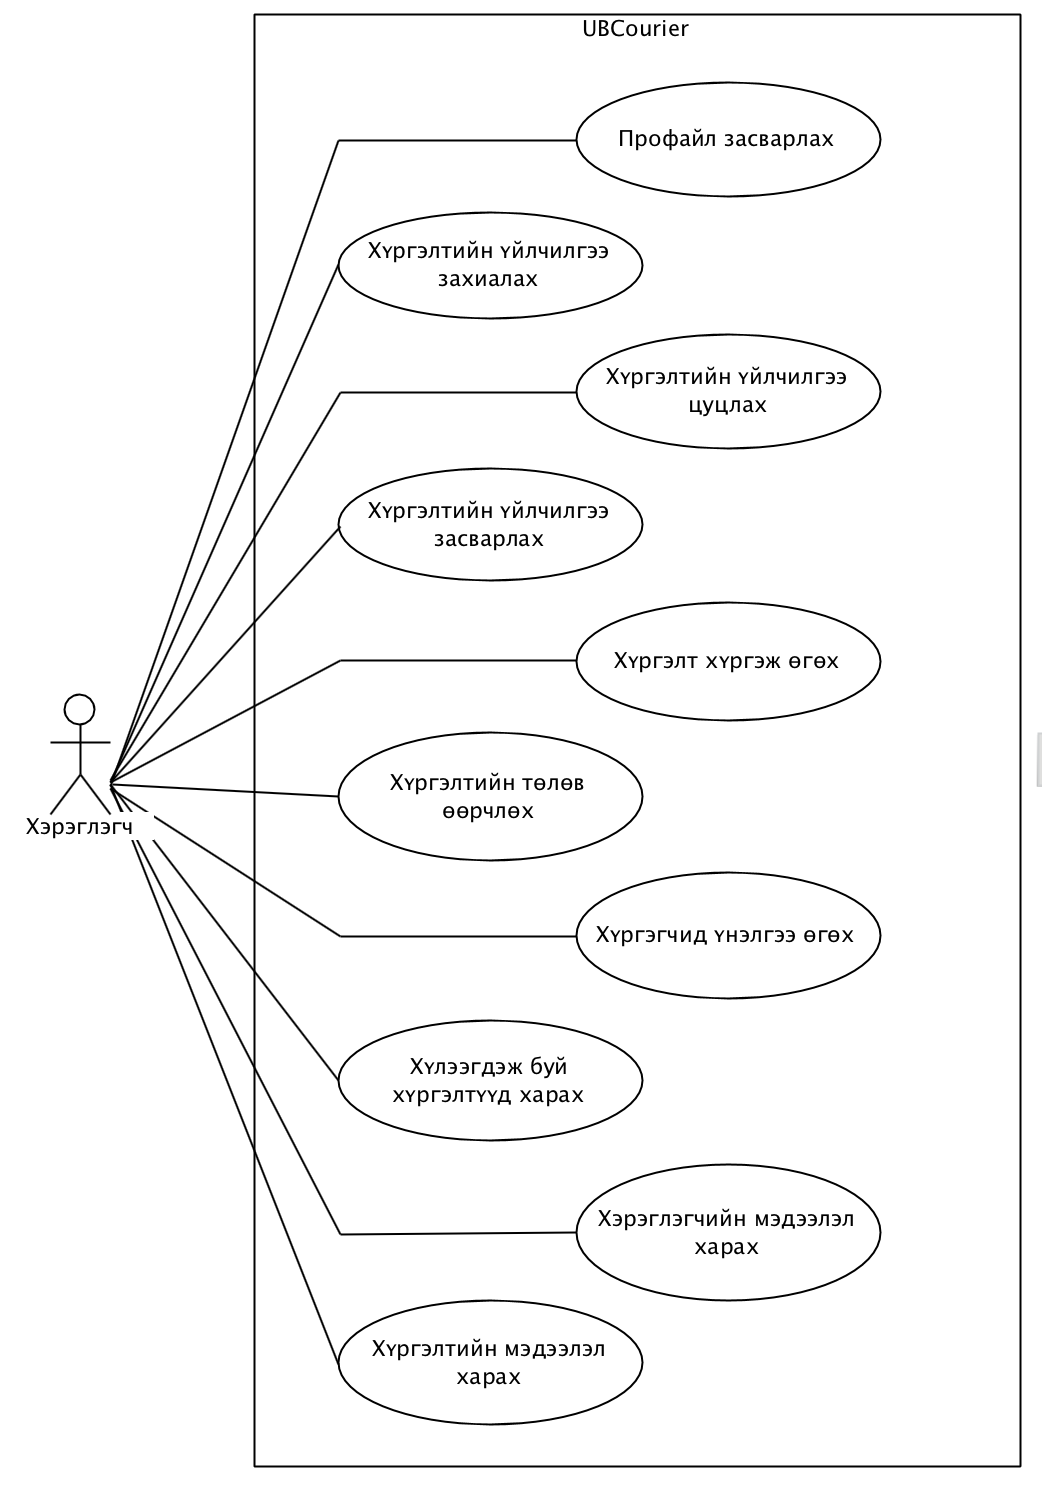
\includegraphics[width=\textwidth]{Figures/shinjilgee/usecase.png}
	\caption{Юзкейс диаграм}
\end{figure}

%-----------------------------------
%	SECTION 6
%-----------------------------------

\section{Юзкейс тодорхойлолт}

\begin{table}[H]
    \caption{Профайл засварлах юзкейс тодорхойлолт}
    \begin{tabular}{|l|p{9cm}|}
		\hline
		{\bfseries Юзкейс:} & Профайл засварлах \\\hline
		{\bfseries ID:} & 1 \\\hline
		{\bfseries Эрэмбэ:} & Өндөр \\\hline
		{\bfseries Үндсэн тоглогч:} & Хэрэглэгч \\\hline
		{\bfseries Нэмэлт тоглогч:} & Байхгүй. \\\hline
		{\bfseries Товч тайлбар:} & Хэрэглэгч өөрийн мэдээллүүдийг засварлах. \\\hline
		{\bfseries Триггер:} & Хэрэглэгч профайл засварлах. \\\hline
		{\bfseries Өмнөх нөхцөл:} & 
		    \begin{enumerate}[nosep]
		        \item Хэрэглэгч өөрийн эрхээр нэвтэрсэн байх.
		        \item Өөрийн профайл руу орсон байх.
		    \end{enumerate}
		\\\hline
		{\bfseries Үндсэн урсгал:} &
			1.0
			\begin{enumerate}[nosep]
				\item IF (Профайл засварлах товчийг дарна)
				    \begin{enumerate}[nosep]
				        \item Бүх мэдээлэл жагсаалт хэлбэрээр гарна.
                        \item Хэрэглэгч мэдээллүүдээ засварлана.
				    \end{enumerate}
				\item IF (Хадгалах товчийг сонговол)
				    \begin{enumerate}[nosep]
				        \item Хэрэглэгчийн мэдээллүүдийг хадгална.
				        \item Хэрэглэгчийн профайл руу буцна.
				    \end{enumerate}
			\end{enumerate}
		\\\hline
		{\bfseries Дараах нөхцөл:} &
		    \begin{enumerate}[nosep]
		        \item Өгөгдлийн санд мэдээллүүдийг хадгална.
		    \end{enumerate}
		\\\hline
		{\bfseries Альтернатив урсгал:} & Байхгүй \\
		\hline
    \end{tabular}
\end{table}

\begin{table}[H]
    \caption{Хүргэлтийн үйлчилгээ захиалах юзкейс тодорхойлолт}
    \begin{tabular}{|l|p{9cm}|}
		\hline
		{\bfseries Юзкейс:} & Хүргэлтийн үйлчилгээ захиалах \\\hline
		{\bfseries ID:} & 2 \\\hline
		{\bfseries Эрэмбэ:} & Өндөр \\\hline
		{\bfseries Үндсэн тоглогч:} & Хэрэглэгч \\\hline
		{\bfseries Нэмэлт тоглогч:} & Байхгүй \\\hline
		{\bfseries Товч тайлбар:} & Шинэ хүргэлт үүсгэх. \\\hline
		{\bfseries Триггер:} & Хэрэглэгч эд зүйл хүргүүлэх хэрэгцээ гарсан. \\\hline
		{\bfseries Өмнөх нөхцөл:} &
		    \begin{enumerate}[nosep]
		        \item Хэрэглэгч өөрийн эрхээр нэвтэрсэн байх.
		        \item Өөрийн хүргэлт цэс рүү орсон байх.
		    \end{enumerate}
		\\\hline
		{\bfseries Үндсэн урсгал:} &
			2.0
			\begin{enumerate}[nosep]
				\item IF (Шинээр хүргэлт үүсгэх товч дээр дарвал)
				    \begin{enumerate}[nosep]
				        \item Хүргэлтийн мэдээллүүд оруулах форм харагдана.
				        \item Хэрэглэгч мэдээллүүдийг бөгөлнө.
				    \end{enumerate}
				\item IF (Хадгалах товч дээр дарвал)
				    \begin{enumerate}[nosep]
				        \item Хүргэлтийн мэдээллүүдийг хадгална.
				        \item Хэрэглэгчийн хүргэлтүүдийн жагсаалт руу буцна.
				    \end{enumerate}
			\end{enumerate}
		\\\hline
		{\bfseries Дараах нөхцөл:} &
		    \begin{enumerate}[nosep]
		        \item Өгөгдлийн санд хүргэлтийг хадгална.
		        \item Шинэ хүргэлт нэмэгдэнэ.
		    \end{enumerate}
		\\\hline
		{\bfseries Альтернатив урсгал:} & Байхгүй
		\\\hline
    \end{tabular}
\end{table}

\begin{table}[H]
    \caption{Хүргэлтийн үйлчилгээ цуцлах юзкейс тодорхойлолт}
    \begin{tabular}{|l|p{9cm}|}
		\hline
		{\bfseries Юзкейс:} & Хүргэлтийн үйлчилгээ цуцлах \\\hline
		{\bfseries ID:} & 3 \\\hline
		{\bfseries Эрэмбэ:} & Өндөр \\\hline
		{\bfseries Үндсэн тоглогч:} & Хэрэглэгч \\\hline
		{\bfseries Нэмэлт тоглогч:} & Байхгүй \\\hline
		{\bfseries Товч тайлбар:} & Хүргэлт устгах.\\\hline
		{\bfseries Триггер:} & Хэрэглэгч хүргэлт устгах хэрэгцээ гарсан. \\\hline
		{\bfseries Өмнөх нөхцөл:} &
		    \begin{enumerate}[nosep]
		        \item Хэрэглэгч өөрийн эрхээр нэвтэрсэн байх.
		        \item Устгахын тулд хүргэлт үүсгэсэн байх.
		    \end{enumerate}
		\\\hline
		{\bfseries Үндсэн урсгал:} &
			3.0
			\begin{enumerate}[nosep]
				\item IF (Өөрийн үүсгэсэн хүртгэлт засварлах дээр дарвал)
				    \begin{enumerate}[nosep]
				        \item Хүргэлтийн мэдээллүүд харагдана.
				        \item IF (Хэрэглэгч хүргэлт устгах товч дээр дарвал.)
                        \begin{enumerate}[nosep]
                            \item Хэрэглэгчийн хүргэлтүүдийн жагсаалтруу буцна.
                            \item Хэрэглэгчийн усгахыг хүссэн хүргэлт устана.
                        \end{enumerate}
				    \end{enumerate}
			\end{enumerate}
		\\\hline
		{\bfseries Дараах нөхцөл:} &
		    \begin{enumerate}[nosep]
		        \item Өгөгдлийн сангаас хүргэлтийг устгана.
		        \item Хэрэглэгчийн усгахыг хүссэн хүргэлт устана.
		    \end{enumerate}
		\\\hline
		{\bfseries Альтернатив урсгал:} & Байхгүй
		\\\hline
    \end{tabular}
\end{table}

\begin{table}[H]
    \caption{Хүргэлтийн үйлчилгээ засварлах юзкейс тодорхойлолт}
    \begin{tabular}{|l|p{9cm}|}
		\hline
		{\bfseries Юзкейс:} & Хүргэлтийн үйлчилгээ засварлах \\\hline
		{\bfseries ID:} & 4 \\\hline
		{\bfseries Эрэмбэ:} & Дунд \\\hline
		{\bfseries Үндсэн тоглогч:} & Хэрэглэгч \\\hline
		{\bfseries Нэмэлт тоглогч:} & Байхгүй \\\hline
		{\bfseries Товч тайлбар:} & Хэрэглэгч өөрийн хүргэлтийн мэдээллээ засварлах.\\\hline
		{\bfseries Триггер:} & Хэрэглэгч өөрийн хүргэлтийн мэдээллээ засварлах хэрэгцээ гарсан. \\\hline
		{\bfseries Өмнөх нөхцөл:} &
		    \begin{enumerate}[nosep]
		        \item Хэрэглэгч өөрийн бүртгэлээр нэвтэрч орсон байх.
		        \item Хэрэглэгчийн засварлах хүргэлтийг хүргэгч хүргэж эхлээгүй байх.
		    \end{enumerate}
		\\\hline
		{\bfseries Үндсэн урсгал:} &
			4.0
			\begin{enumerate}[nosep]
			    \item Хэрэглэгч өөрийн хүргэлтийг засварлах товч дээр дарна.
			    \item Хүргэлтийн мэдээллүүд жагсаалт байдлаар харагдана.
			    \item Хэрэглэгч засварлахыг хүссэн мэдээллүүдээ засна.
				\item IF (Хадгалах дарвал)
				    \begin{enumerate}[nosep]
				        \item Хүргэлтийн мэдээллүүдийг хадгална.
				    \end{enumerate}
			\end{enumerate}
		\\\hline
		{\bfseries Дараах нөхцөл:} &
		    \begin{enumerate}[nosep]
		        \item Хэрэглэгчийн засварласан хүргэлтийн мэдээллийг хадгална.
		        \item Хэрэглэгчийн хүргэлтийн жагсаалтуудыг харуулна.
		    \end{enumerate}
		\\\hline
		{\bfseries Альтернатив урсгал:} & Байхгүй
		\\\hline
    \end{tabular}
\end{table}


\begin{table}[H]
    \caption{Хүргэлт хүргэж өгөх юзкейс тодорхойлолт}
    \begin{tabular}{|l|p{9cm}|}
		\hline
		{\bfseries Юзкейс:} & Хүргэлт хүргэж өгөх \\\hline
		{\bfseries ID:} & 5 \\\hline
		{\bfseries Эрэмбэ:} & Өндөр \\\hline
		{\bfseries Үндсэн тоглогч:} & Хэрэглэгч \\\hline
		{\bfseries Нэмэлт тоглогч:} & Байхгүй \\\hline
		{\bfseries Товч тайлбар:} & Хүргэгч хүргэлтийг авах.\\\hline
		{\bfseries Триггер:} & Хүргэгч хүргэлтийг хүргэж өгөх хүсэлтэй байх. \\\hline
		{\bfseries Өмнөх нөхцөл:} &
		    \begin{enumerate}[nosep]
		        \item Хэрэглэгч өөрийн эрхээр нэвтэрсэн байх.
		        \item Хүргэж өгөх хүргэлт рүү орсон байх.
		    \end{enumerate}
		\\\hline
		{\bfseries Үндсэн урсгал:} &
			6.0
			\begin{enumerate}[nosep]
			    \item Хүргэгчид хүргэлтийн мэдээллүүдийг харуулна.
			    \item Хүргэгч "хүргэж өгөх" товч дээр дарна.
			    \item Хүргэгчийн хүргэлтүүд рүү буцна.
			\end{enumerate}
		\\\hline
		{\bfseries Дараах нөхцөл:} &
		    \begin{enumerate}[nosep]
		        \item Өгөгдлийн санд хүргэлтийг хүргэгч дээр бүртгэнэ.
		    \end{enumerate}
		\\\hline
		{\bfseries Альтернатив урсгал:} & Байхгүй
		\\\hline
    \end{tabular}
\end{table}

\begin{table}[H]
    \caption{Хүргэгчид үнэлгээ өгөх юзкейс тодорхойлолт}
    \begin{tabular}{|l|p{9cm}|}
		\hline
		{\bfseries Юзкейс:} & Хүргэгчид үнэлгээ өгөх \\\hline
		{\bfseries ID:} & 7 \\\hline
		{\bfseries Эрэмбэ:} & Өндөр \\\hline
		{\bfseries Үндсэн тоглогч:} & Хэрэглэгч \\\hline
		{\bfseries Нэмэлт тоглогч:} & Байхгүй \\\hline
		{\bfseries Товч тайлбар:} & Хүргэлтийн үйлчилгээ захиалсан хэрэглэгч хүргэгчид үнэлгээ өгөх.\\\hline
		{\bfseries Триггер:} & Хүргэгч хүргэлтийг очих ёстой газар нь хүргэсэн байх. \\\hline
		{\bfseries Өмнөх нөхцөл:} &
		    \begin{enumerate}[nosep]
		        \item Хэрэглэгч өөрийн эрхээр нэвтэрсэн байх.
		        \item Хүргэж өгсөн хүргэлт рүү орсон байх.
		    \end{enumerate}
		\\\hline
		{\bfseries Үндсэн урсгал:} &
			7.0
			\begin{enumerate}[nosep]
			    \item Хүргэлтийн мэдээллүүдийг харуулна.
			    \item Хэрэглэгч хүргэгчид үнэлгээ өгөх товчийг дарна.
			    \item Хэрэглэгчид үнэлгээ өгөх цонхийг харуулна.
			    \item Хэрэглэгч хүргэгчид үнэлгээг 1-5 одоор мөн текстээр өгнө.
			\end{enumerate}
		\\\hline
		{\bfseries Дараах нөхцөл:} &
		    \begin{enumerate}[nosep]
		        \item Өгөгдлийн санд үнэлгээг хадгална.
		        \item Хүргэлтүүдийн жагсаалт руу буцна.
		    \end{enumerate}
		\\\hline
		{\bfseries Альтернатив урсгал:} & Байхгүй
		\\\hline
    \end{tabular}
\end{table}

\begin{table}[H]
    \caption{Хүлээгдэж буй хүргэлтүүд харах юзкейс тодорхойлолт}
    \begin{tabular}{|l|p{9cm}|}
		\hline
		{\bfseries Юзкейс:} & Хүлээгдэж буй хүргэлтүүд харах \\\hline
		{\bfseries ID:} & 8 \\\hline
		{\bfseries Эрэмбэ:} & Өндөр \\\hline
		{\bfseries Үндсэн тоглогч:} & Хэрэглэгч \\\hline
		{\bfseries Нэмэлт тоглогч:} & Байхгүй \\\hline
		{\bfseries Товч тайлбар:} & Хүргэгч хүргэж эхлээгүй хүлээгдэж буй хүргэлтүүд харах. \\\hline
		{\bfseries Триггер:} & Хүргэгч хүлээгдэж буй хүргэлтүүдийг харах хүсэлтэй байх. \\\hline
		{\bfseries Өмнөх нөхцөл:} &
		    \begin{enumerate}[nosep]
		        \item Хэрэглэгч өөрийн эрхээр нэвтэрсэн байх.
		        \item Цэснээс нүүр цэсийг сонгох.
		    \end{enumerate}
		\\\hline
		{\bfseries Үндсэн урсгал:} &
			8.0
			\begin{enumerate}[nosep]
				\item IF (Хүлээгдэж буй хүргэлтүүд байвал)
				    \begin{enumerate}[nosep]
		                \item Хүлээгдэх буй хүргэлтүүдийг харуулна.
				    \end{enumerate}
				\item ELSE
				    \begin{enumerate}[nosep]
		                \item Юу ч харуулахгүй.
				    \end{enumerate}
			\end{enumerate}
		\\\hline
		{\bfseries Дараах нөхцөл:} & Байхгүй \\\hline
		{\bfseries Альтернатив урсгал:} & Байхгүй \\\hline
    \end{tabular}
\end{table}

\begin{table}[H]
    \caption{Хэрэглэгчийн мэдээлэл харах юзкейс тодорхойлолт}
    \begin{tabular}{|l|p{9cm}|}
		\hline
		{\bfseries Юзкейс:} & Хэрэглэгчийн мэдээлэл харах \\\hline
		{\bfseries ID:} & 9 \\\hline
		{\bfseries Эрэмбэ:} & Өндөр \\\hline
		{\bfseries Үндсэн тоглогч:} & Хэрэглэгч \\\hline
		{\bfseries Нэмэлт тоглогч:} & Байхгүй \\\hline
		{\bfseries Товч тайлбар:} & Хэрэглэгчийн профайл харах. \\\hline
		{\bfseries Триггер:} & Хэрэглэгч бусад хэрэглэгчийн мэдээллүүдийг харах хүсэлтэй байх. \\\hline
		{\bfseries Өмнөх нөхцөл:} &
		    \begin{enumerate}[nosep]
		        \item Хэрэглэгч өөрийн эрхээр нэвтэрсэн байх.
		        \item Ямар нэг хүргэлтийн мэдээлэл рүү орсон байх.
		    \end{enumerate}
		\\\hline
		{\bfseries Үндсэн урсгал:} &
			9.0
			\begin{enumerate}[nosep]
				\item IF (Хэрэглэгчийн нэр эсвэл зураг дээр дарвал)
				    \begin{enumerate}[nosep]
		                \item Хэрэглэгчийн профайл болон бусад мэдээллүүдийг харуулна.
				    \end{enumerate}
			\end{enumerate}
		\\\hline
		{\bfseries Дараах нөхцөл:} & Байхгүй \\\hline
		{\bfseries Альтернатив урсгал:} & Байхгүй \\\hline
    \end{tabular}
\end{table}

\begin{table}[H]
    \caption{Хүргэлтийн мэдээлэл харах юзкейс тодорхойлолт}
    \begin{tabular}{|l|p{9cm}|}
		\hline
		{\bfseries Юзкейс:} & Хүргэлтийн мэдээлэл харах \\\hline
		{\bfseries ID:} & 10 \\\hline
		{\bfseries Эрэмбэ:} & Өндөр \\\hline
		{\bfseries Үндсэн тоглогч:} & Хэрэглэгч \\\hline
		{\bfseries Нэмэлт тоглогч:} & Байхгүй \\\hline
		{\bfseries Товч тайлбар:} & Хүргэлтийн мэдээлэл харах. \\\hline
		{\bfseries Триггер:} & Хэрэглэгч бусад хүргэлтийн мэдээллүүдийг харах хүсэлтэй байх. \\\hline
		{\bfseries Өмнөх нөхцөл:} &
		    \begin{enumerate}[nosep]
		        \item Хэрэглэгч өөрийн эрхээр нэвтэрсэн байх.
		        \item Нүүр цэсийг сонгосон байх.
		    \end{enumerate}
		\\\hline
		{\bfseries Үндсэн урсгал:} &
			10.0
			\begin{enumerate}[nosep]
				\item IF (Хэрэглэгч нэг хүргэлт дээр дарвал)
				    \begin{enumerate}[nosep]
		                \item Хүргэлтийн мэдээллүүдийг харуулна.
				    \end{enumerate}
			\end{enumerate}
		\\\hline
		{\bfseries Дараах нөхцөл:} & Байхгүй \\\hline
		{\bfseries Альтернатив урсгал:} & Байхгүй \\\hline
    \end{tabular}
\end{table}

%-----------------------------------
%	SECTION 7
%-----------------------------------

\section{Шинжилгээнии класс диаграм}

\begin{figure}[H]
    \centering
	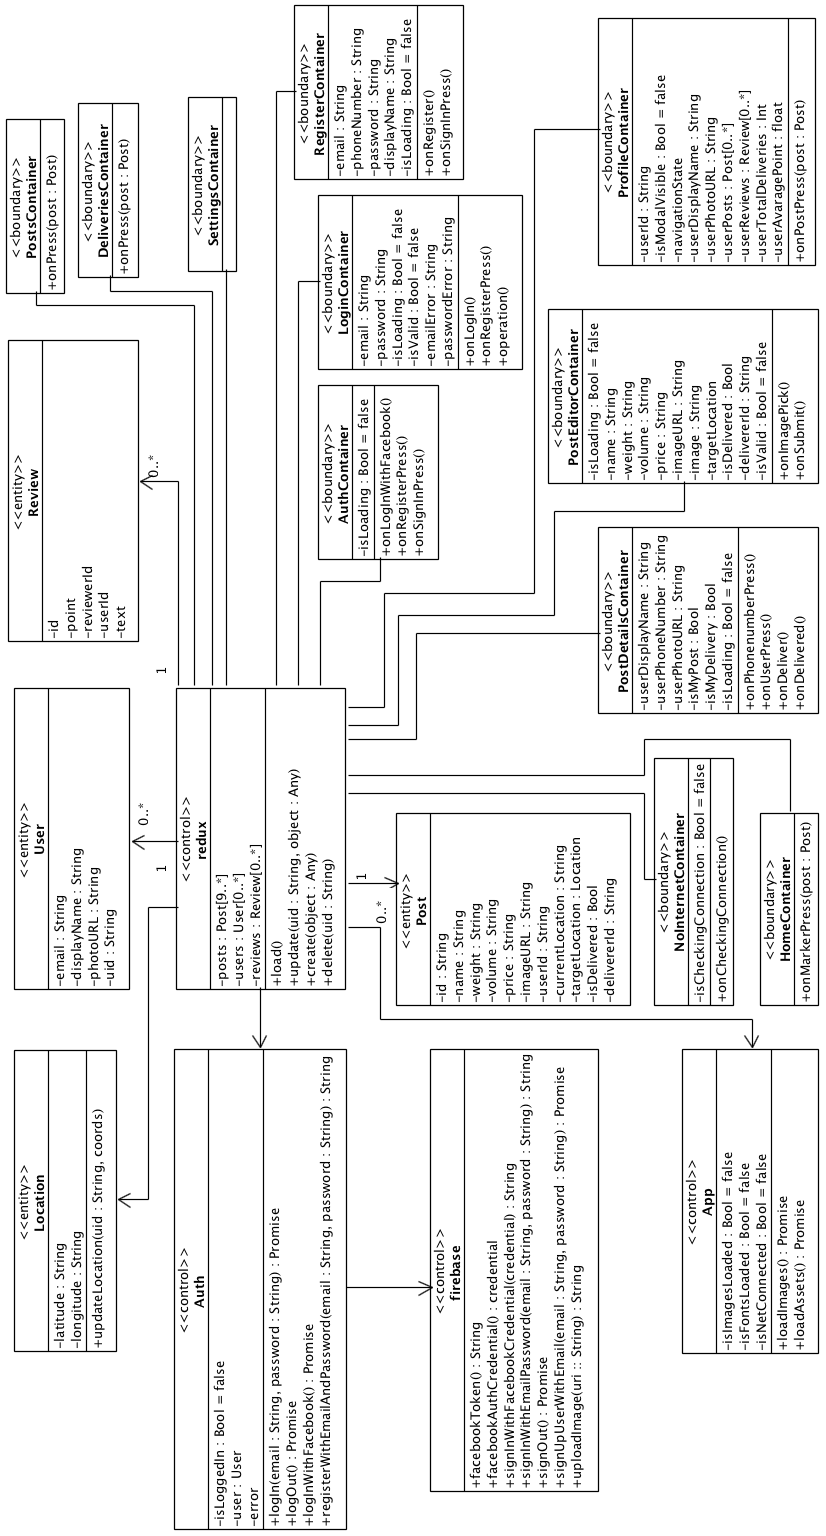
\includegraphics[height=.88\textheight]{Figures/shinjilgee/class_diagram.png}
	\caption{Шинжилгээнии класс диаграм}
\end{figure}

%-----------------------------------
%	SECTION 8
%-----------------------------------

\section{Шинжилгээний дарааллын диаграм}

\begin{figure}[H]
	\centering
	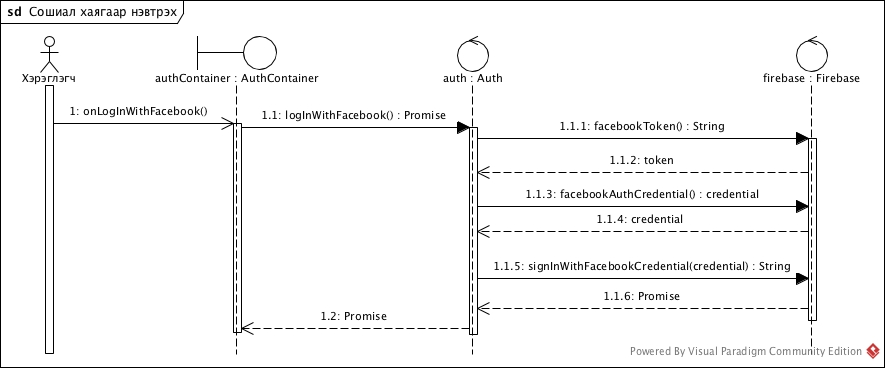
\includegraphics[width=\textwidth]{Figures/shinjilgee/seq/social_haygaar_nevtreh.jpg}
	\caption{Сошиал хаягаар нэвтрэх дарааллын диаграм}
\end{figure}

\begin{figure}[H]
	\centering
	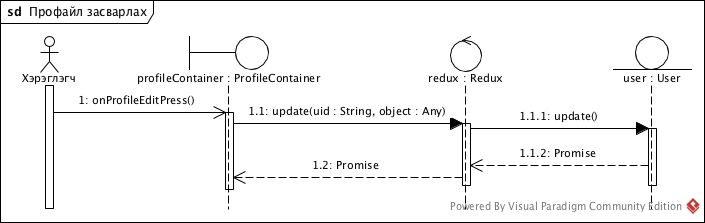
\includegraphics[width=\textwidth]{Figures/shinjilgee/seq/profile_zasvarlah.jpg}
  \caption{Профайл засварлах дарааллын диаграм}
\end{figure}

\begin{figure}[H]
	\centering
	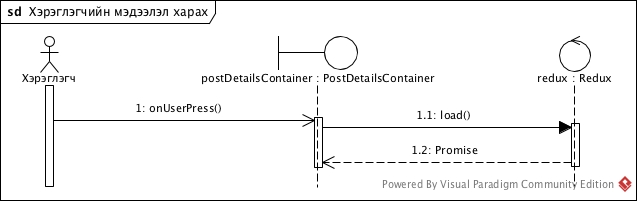
\includegraphics[width=\textwidth]{Figures/shinjilgee/seq/test.jpg}
  \caption{Хэрэглэгчийн мэдээлэл харах дарааллын диаграм}
\end{figure}

\begin{figure}[H]
	\centering
	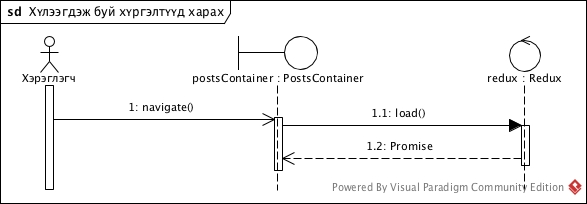
\includegraphics[width=\textwidth]{Figures/shinjilgee/seq/huleegdej_bui_hurgelt_harah.jpg}
  \caption{Хүлээгдэж буй хүргэлтүүд харах дарааллын диаграм}
\end{figure}

\begin{figure}[H]
	\centering
	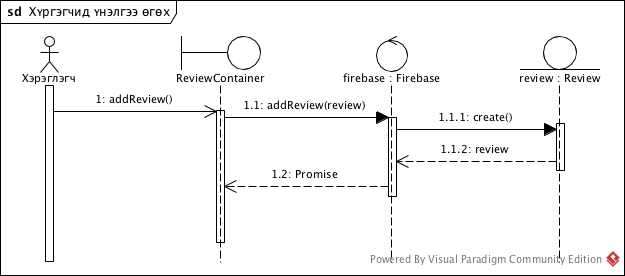
\includegraphics[width=\textwidth]{Figures/shinjilgee/seq/hurgegchid_unelgee_ogoh.jpg}
  \caption{Хүргэгчид үнэлгээ өгөх дарааллын диаграм}
\end{figure}

\begin{figure}[H]
	\centering
	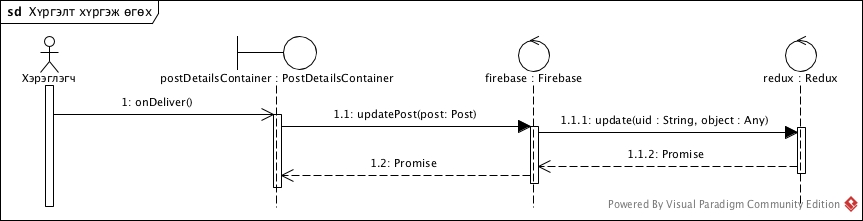
\includegraphics[width=\textwidth]{Figures/shinjilgee/seq/hurgelt_hurgej_ogoh.jpg}
  \caption{Хүргэлт хүргэж өгөх дарааллын диаграм}
\end{figure}

\begin{figure}[H]
	\centering
	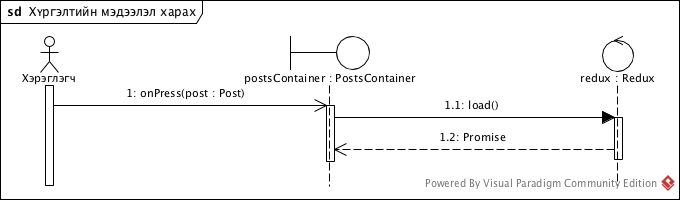
\includegraphics[width=\textwidth]{Figures/shinjilgee/seq/hurgeltiin_medeelel_harah.jpg}
  \caption{Хүргэлтийн мэдээлэл харах дарааллын диаграм}
\end{figure}

\begin{figure}[H]
	\centering
	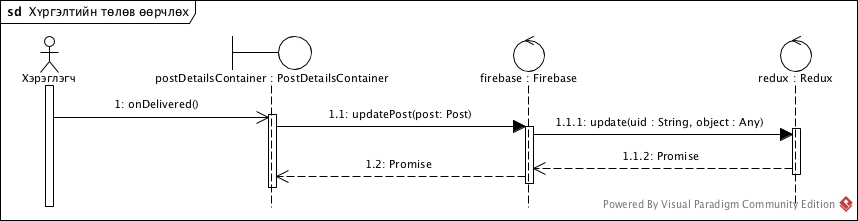
\includegraphics[width=\textwidth]{Figures/shinjilgee/seq/hurgeltiin_tolov_oorchloh.jpg}
  \caption{Хүргэлтийн төлөв өөрчлөх дарааллын диаграм}
\end{figure}

\begin{figure}[H]
	\centering
	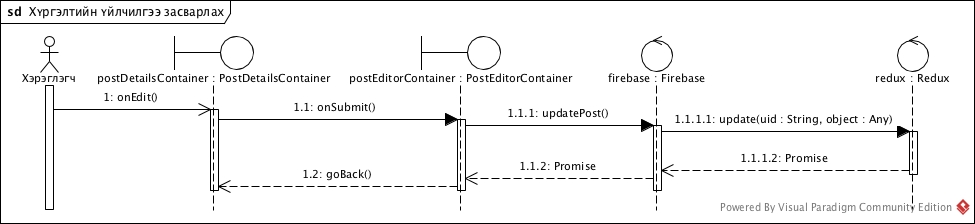
\includegraphics[width=\textwidth]{Figures/shinjilgee/seq/hurgeltiin_uilchilgee_zasvarlah.jpg}
  \caption{Хүргэлтийн үйлчилгээ засварлах дарааллын диаграм}
\end{figure}

\begin{figure}[H]
	\centering
	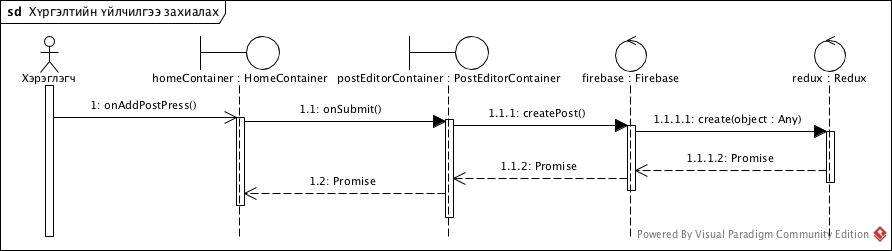
\includegraphics[width=\textwidth]{Figures/shinjilgee/seq/hurgeltiin_uilchilgee_zahialah.jpg}
  \caption{Хүргэлтийн үйлчилгээ захиалах дарааллын диаграм}
\end{figure}

\begin{figure}[H]
	\centering
	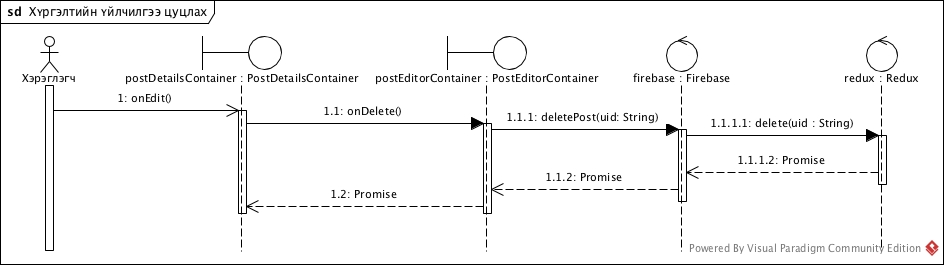
\includegraphics[width=\textwidth]{Figures/shinjilgee/seq/hurgeltiin_uilchilgee_tsutslah.jpg}
  \caption{Хүргэлтийн үйлчилгээ цуцлах дарааллын диаграм}
\end{figure}

%-----------------------------------
%	SECTION 9
%-----------------------------------

\section{Үйл ажиллагааны диаграм}

\begin{figure}[H]
  \centering
	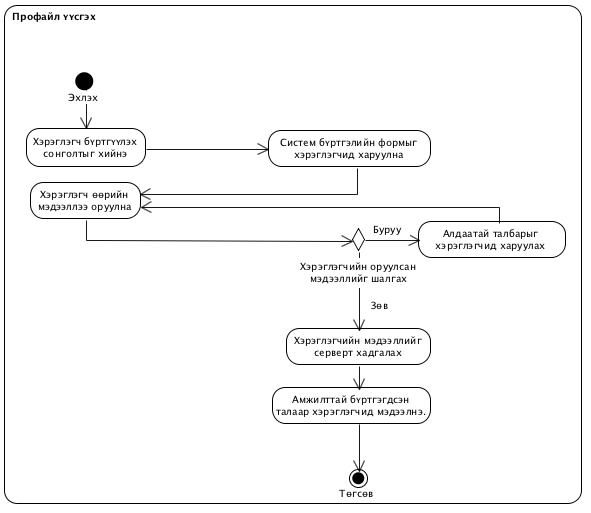
\includegraphics[width=\textwidth]{Figures/shinjilgee/activity/profile_uusgeh.png}
	\caption{Профайл үүсгэх үйл ажиллагааны диаграм}
\end{figure}

\begin{figure}[H]
  \centering
	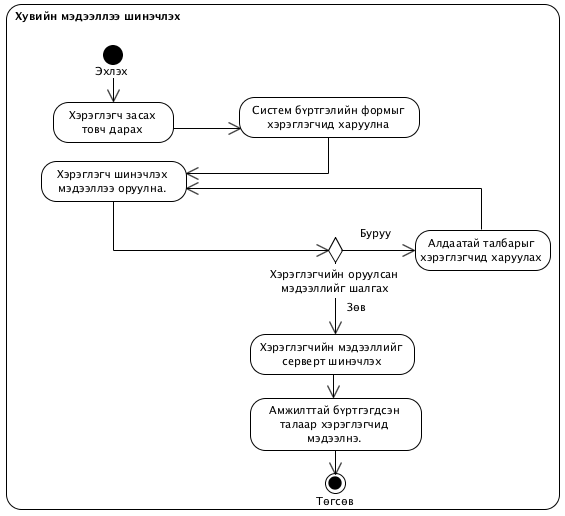
\includegraphics[width=\textwidth]{Figures/shinjilgee/activity/huviin_medeellee_shinchleh.png}
	\caption{Хувийн мэдээллээ шинэчлэх үйл ажиллагааны диаграм}
\end{figure}

\begin{figure}[H]
  \centering
	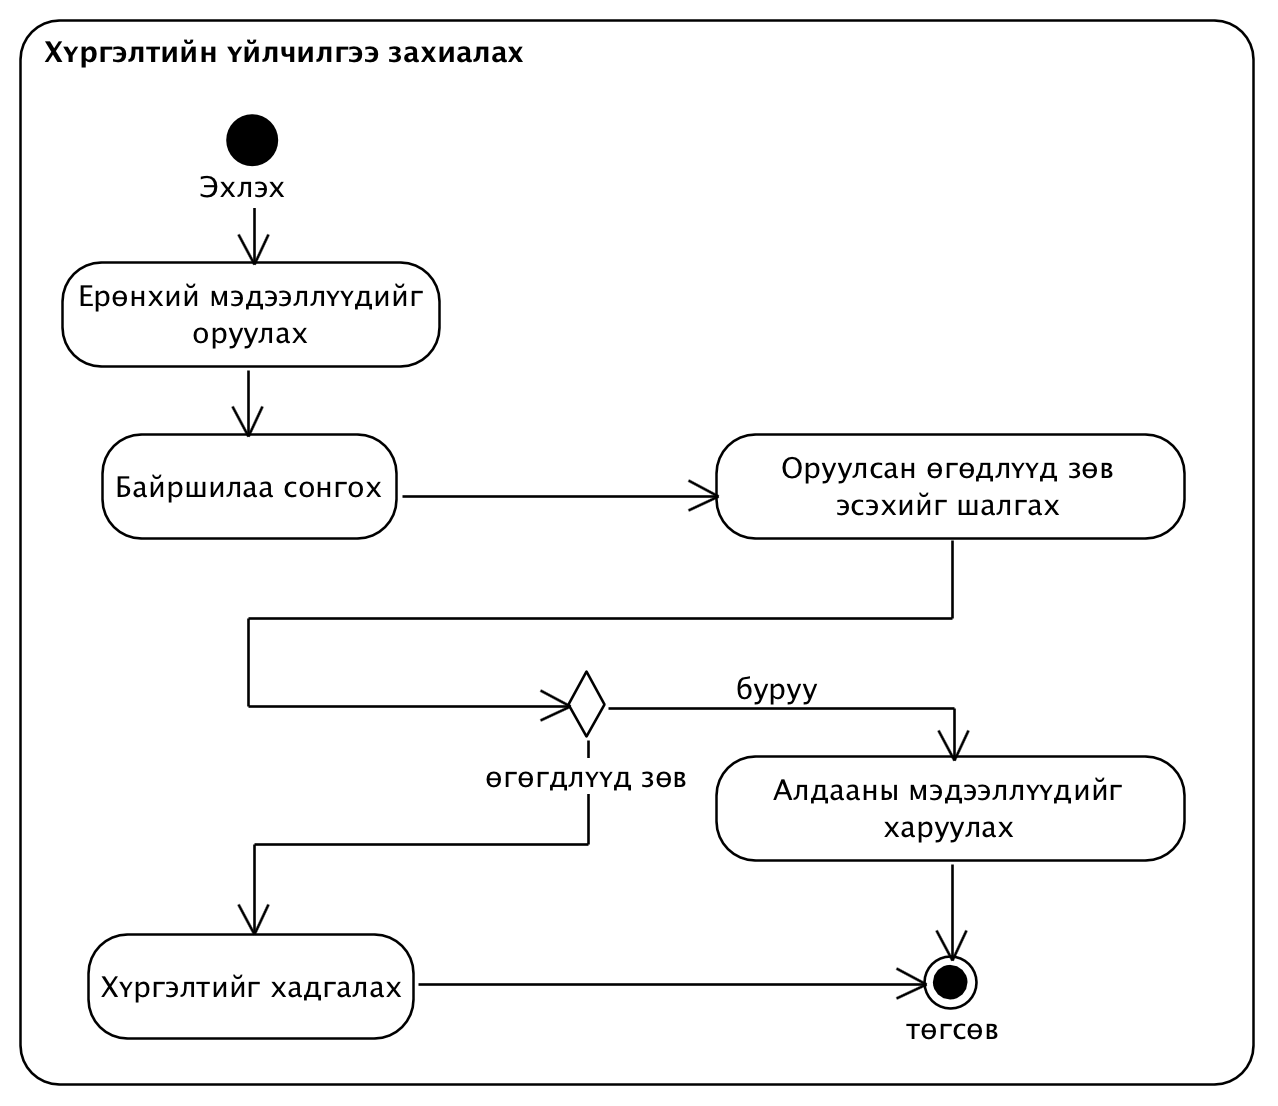
\includegraphics[width=\textwidth]{Figures/shinjilgee/activity/hurgeltiin_uilchilgee_zahialah.png}
	\caption{Хүргэлтийн үйлчилгээ захиалах үйл ажиллагааны диаграм}
\end{figure}

\begin{figure}[H]
  \centering
	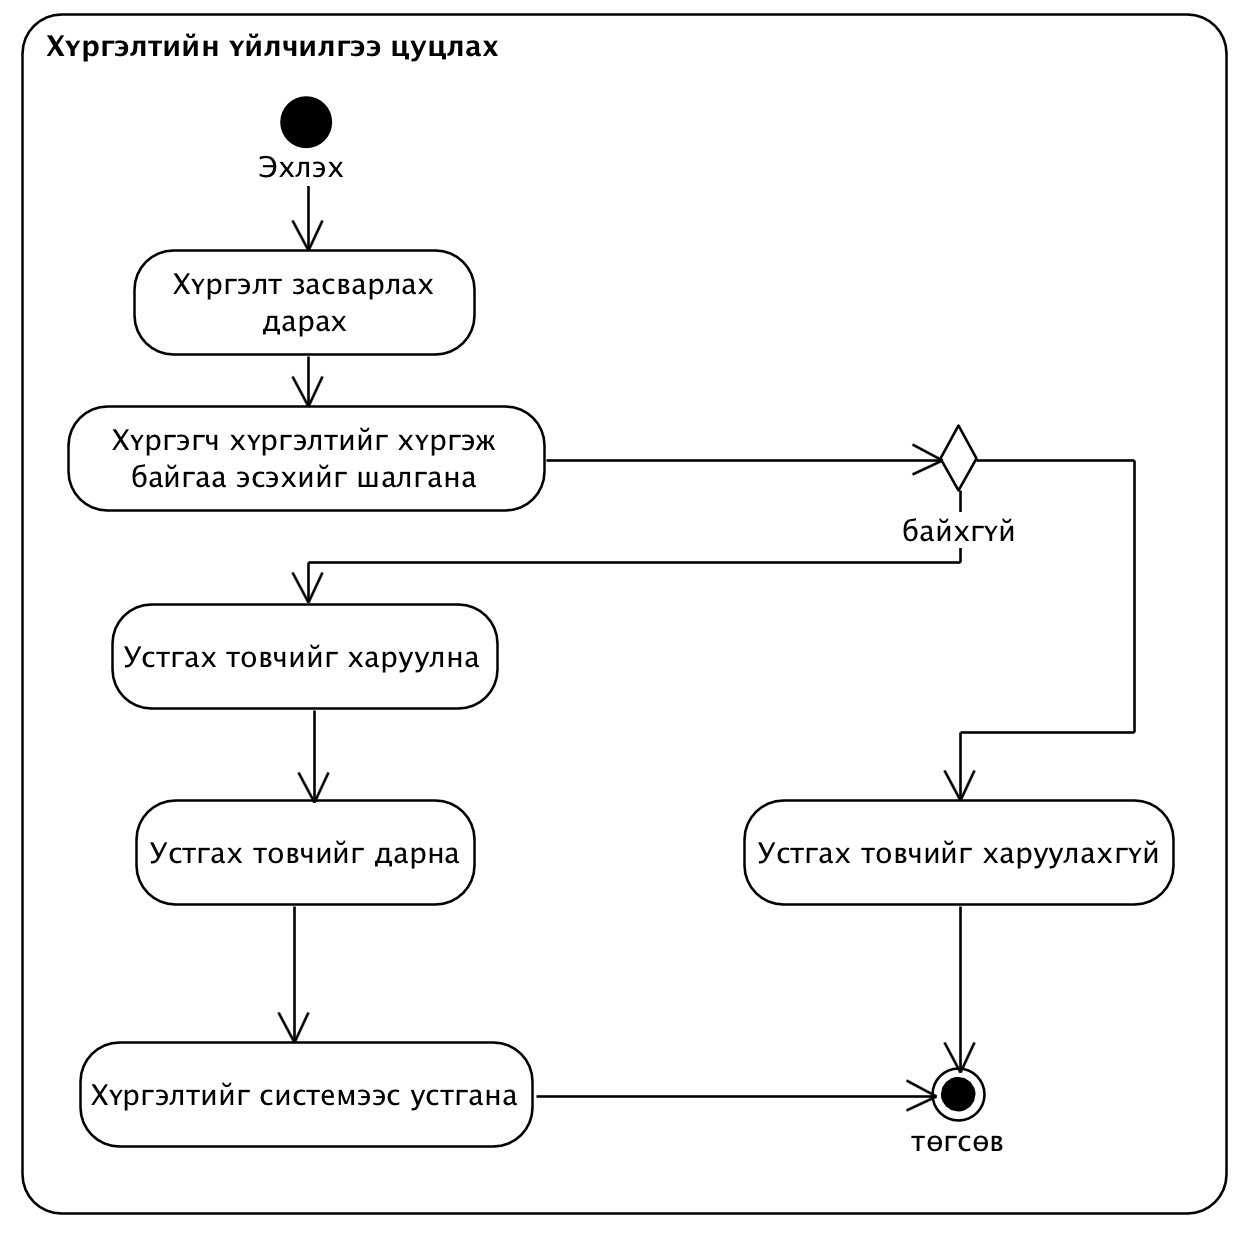
\includegraphics[width=\textwidth]{Figures/shinjilgee/activity/hurgeltiin_uilchilgee_tsutslah.png}
	\caption{Хүргэлтийн үйлчилгээ цуцлах үйл ажиллагааны диаграм}
\end{figure}

\begin{figure}[H]
  \centering
	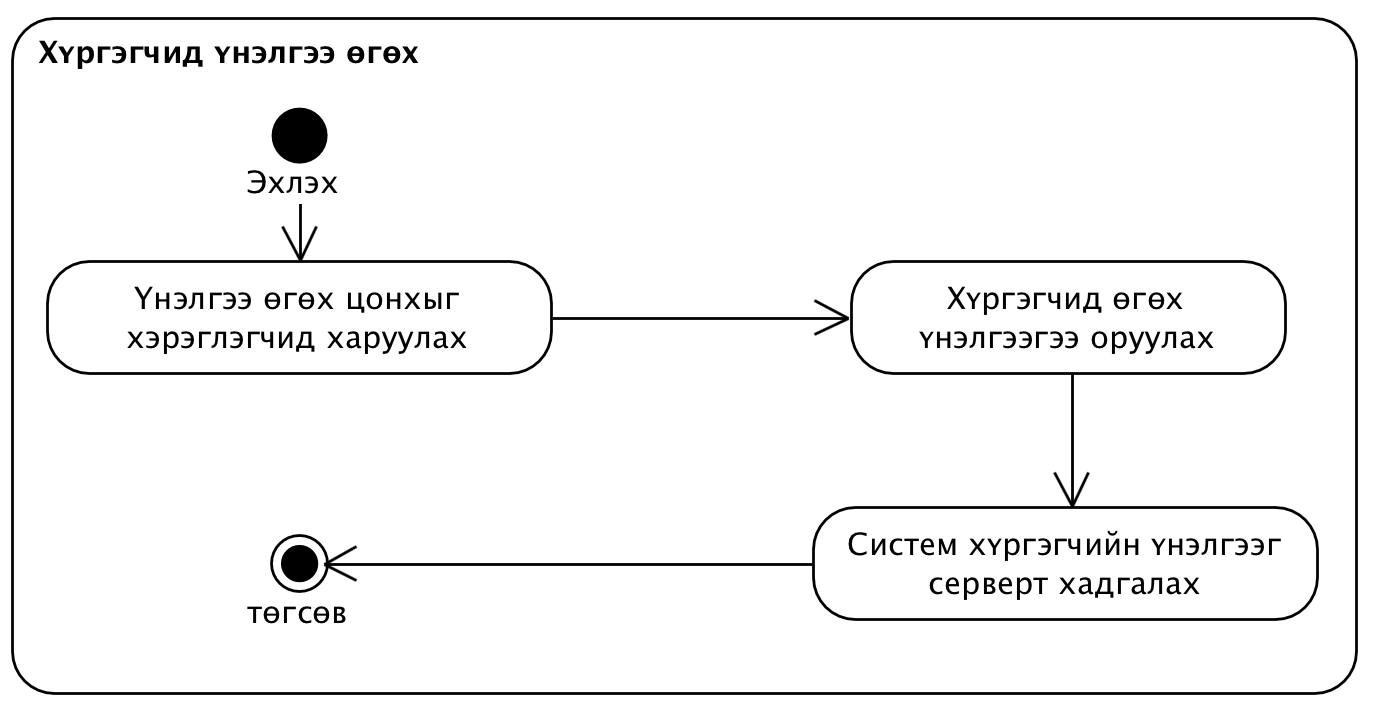
\includegraphics[width=\textwidth]{Figures/shinjilgee/activity/hurgegchid_unelgee_ogoh.png}
	\caption{Хүргэгчид үнэлгээ өгөх үйл ажиллагааны диаграм}
\end{figure}

\begin{figure}[H]
  \centering
	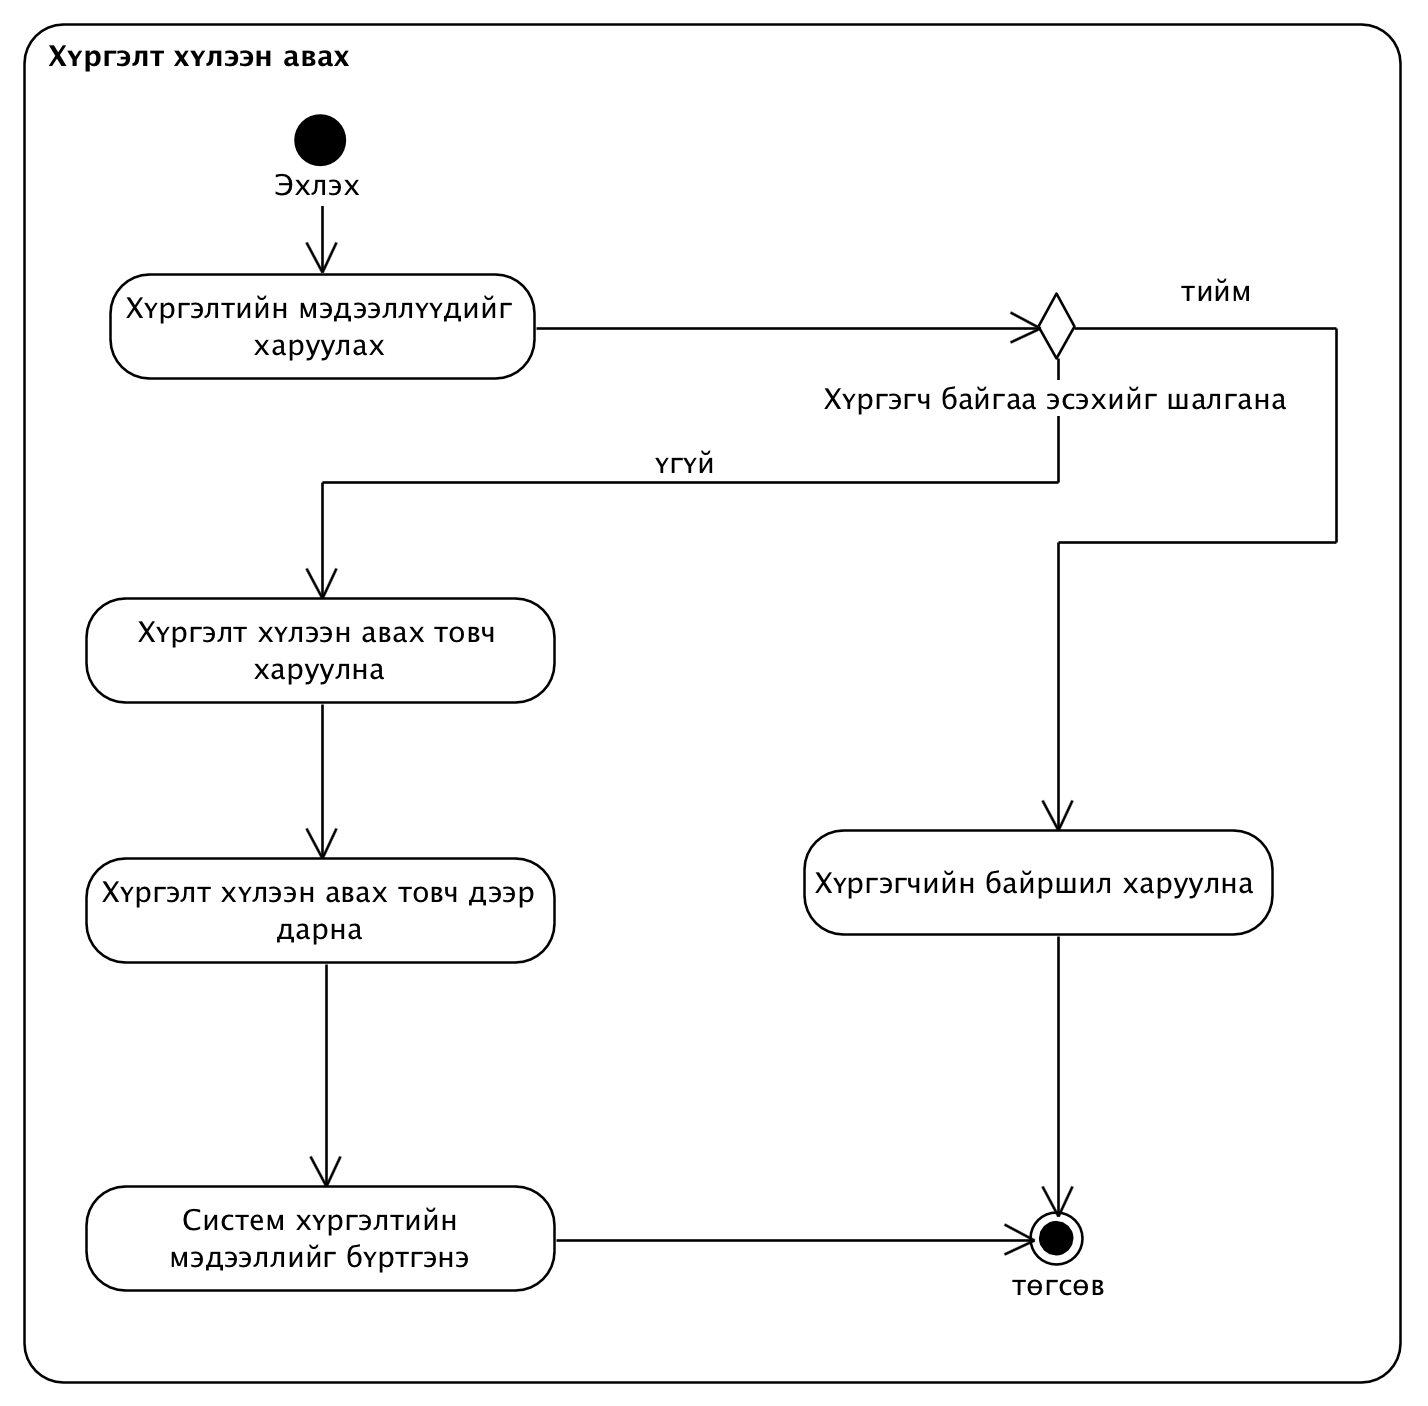
\includegraphics[width=\textwidth]{Figures/shinjilgee/activity/hurgelt_huleen_avah.png}
	\caption{Хүргэлт хүлээн авах үйл ажиллагааны диаграм}
\end{figure}

\begin{figure}[H]
  \centering
	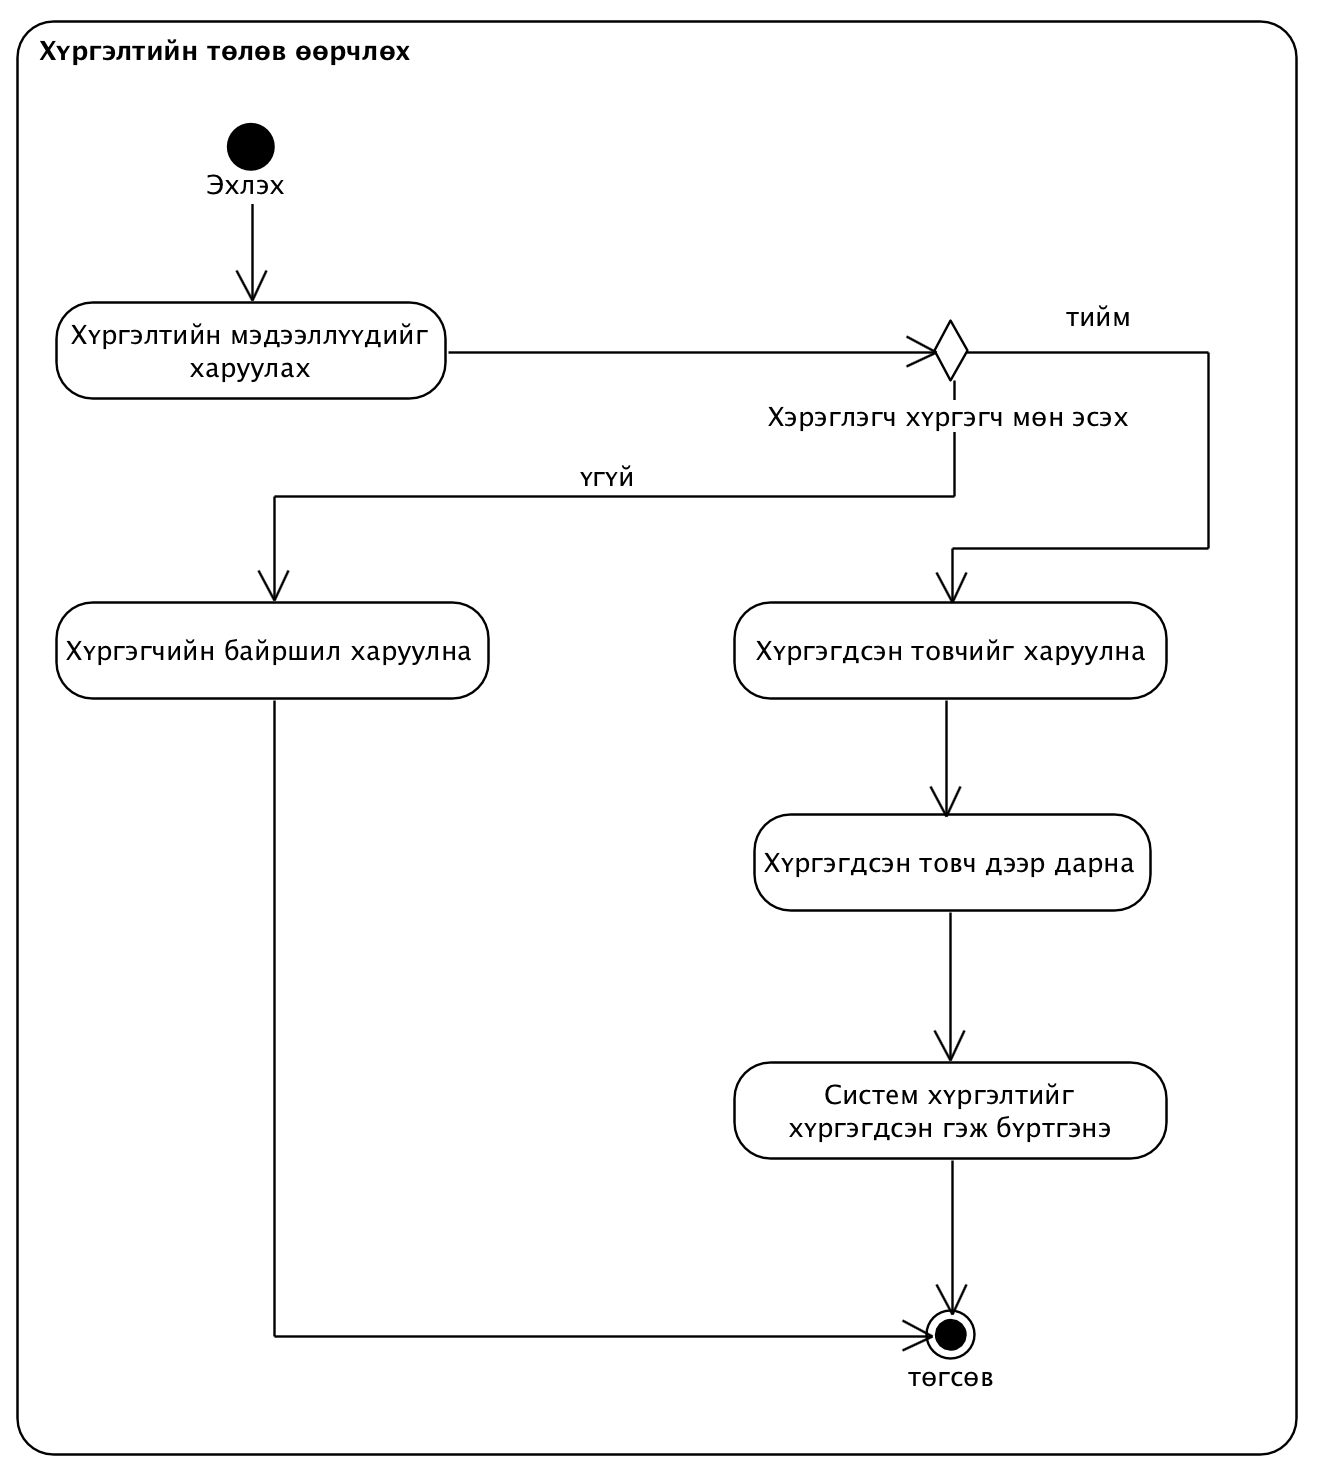
\includegraphics[width=\textwidth]{Figures/shinjilgee/activity/hurgeltiin_tolov_oorchloh.png}
	\caption{Хүргэлтийн төлөв өөрчлөх үйл ажиллагааны диаграм}
\end{figure}

%-----------------------------------
%	SECTION 10
%-----------------------------------

\section{Бүлгийн дүгнэлт}
Энэ бүлгийн хүрээнд уг системийн шаардлага болон шинжилгээний шатны бичиг баримтыг хийж гүйцэтгэсэн ба дараах зүйлсийг тодорхойлов:
\begin{itemize}[label={--}]
    \renewcommand\labelitemi{--}
    \item Системийн үйл ажиллагааг тодорхойлсон,
    \item Системийг ашиглах хэрэглэгчдийг тодорхойлсон,
    \item Функцийн шаардлагуудыг тодорхойлсон,
    \item Функцийн бус шаардлагуудыг тодорхойлсон,
    \item Юзкейс диаграмыг тодорхойлсон,
    \item Юзкейс тодорхойлолтуудыг тодорхойлсон,
    \item Шинжилгээний класс диаграмыг дүрсэлсэн,
    \item Шинжилгээний дарааллын диаграмыг дүрсэлсэн,
    \item Үйл ажиллагааны диаграмыг гаргасан болно.
\end{itemize}